\section{Domain Name System}\label{sec:background_dns}

\dns, a key component of Internet infrastructure and connectivity, is a hierarchical system responsible for converting domain names to \ip addresses. Domain names are human-readable names used to identify servers and websites. They are easier to remember than \ip addresses, and can point to more than one address depending on geographic location or load-balancing constraints to provide higher-performance access to websites for end-users. Domain names contain one or more parts called \textit{labels}, separated by dots. The rightmost label is the \tld (e.g. \texttt{com}, \texttt{org}, \texttt{net}, etc.). The \dns hierarchy tree subdivides into "zones," with each zone containing one or more domain names and sub-domains. Databases of domain names are maintained by \dns Name Servers, which resolve domains to \ip addresses  (\cref{fig:dns_resolution}). There are two types of name servers: authoritative and recursive.

Beyond caching resources that the end user sees and interacts with, other things, like \dns results, use caching as well. As discussed in more detail in \autoref{sec:background_dns}, recursive \dns servers retrieve requests from other \dns servers and often cache them for responding to future requests \cite{rfc1035}. Similar to the expiration time  in HTTP caching, \dns caching has a \ttl that for

\begin{wrapfigure}[18]{R}{0.4\textwidth}
    \centering
    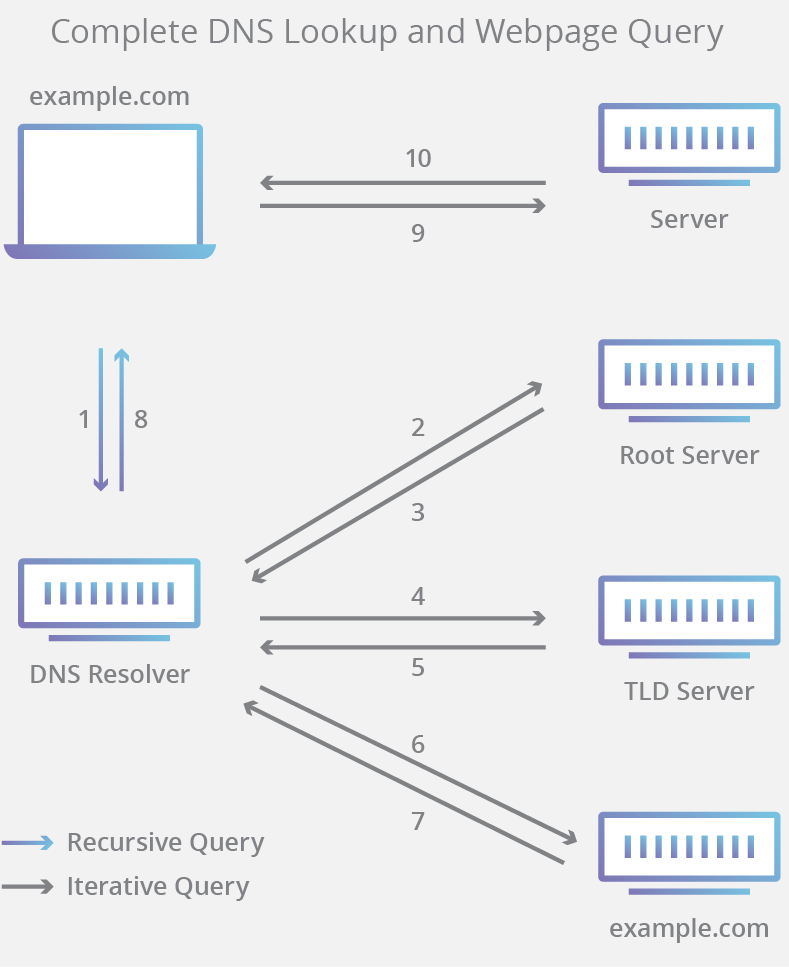
\includegraphics[width=0.4\textwidth]{images/other/dns_lookup_diagram.png}
    \caption{Diagram of DNS resolution \cite{Cloudflare2020a}}
    \label{fig:dns_resolution}
\end{wrapfigure}

\subsection{Authoritative Servers}
Authoritative servers are the primary source for the domain names within a given zone. When querying for any domain, the answer will ultimately come from the authoritative server for that domain. A \dns client can query an authoritative server directly, but it is more common that an authoritative server will be queried by a recursive server on behalf of a \dns client.

\subsection{Recursive Servers}
Recursive \dns servers work to find an \ip address for a client, so that the client does not have to do the leg work of searching through other \dns servers \cite{Cloudflarea}. \DNS resolvers use a predetermined upstream recursive \dns server, such as one provided by an \isp \cite{Oracle2010RecursiveWork}. This server then checks its cache and, if it has a valid answer, returns it. Otherwise, the server makes a series of iterative queries in order to find the requested name. 

Take for example, \texttt{www.google.com}. If the recursive server has no knowledge of any parts of the \acUrl, it will first query a pre-configured root \dns server for the authoritative server for the \texttt{.com} \tld. It will then query that server for \texttt{google.com}, then query the server provided from that request for \texttt{www.google.com} itself. At this point, the iterative component of the lookup is complete. At each stage of this process, the recursive server caches the results of its query, and assuming the \ttl has not expired, will use that cached value instead of making a fresh query. Finally, the recursive server then returns the \ip address it located, completing the recursive request from the user.

\subsection{Public Recursive \dns Servers}
An important part of this project involves public recursive \dns servers. These servers are \dns servers configured to respond to requests from anyone. Whereas most \isp servers do not advertise their \dns servers to non-customers, public servers do. Some organizations, like Google and CloudFlare, provide public \dns services because they believe doing so improves the browsing experience for end users \cite{GoogleIntroductionDNS}. These provide the public with \dns options outside of their \isp and provide this project with an important set of geographically diverse servers.
